% Пример статьи для журнала КИО
% Кодировка файла должна быть UTF-8.
\documentclass[intlimits,twoside,a4paper,11pt]{article}

\usepackage{amsmath,amssymb,amsthm}

\usepackage[eqsecnum,authorsinfo]{kioj6}

\usepackage{enumitem}
\usepackage{booktabs}
\usepackage{caption}
\usepackage{float}
\usepackage{listings}
\usepackage{xcolor}
\usepackage{graphicx}
\usepackage{url}

\theoremstyle{definition}
\newtheorem{definition}{Определение}[section]
\newtheorem{theorem}{Теорема}[section]

% ===================== НАСТРОЙКИ ЖУРНАЛА ====================

\setcounter{page}{1}

\journalsectionnoimage{empty}
\issue{2026}{--}{edu}
\articletype{1}

\udknumber{999.999}

\doinumber{10.32603/2071-2340-XXX}

% =============== РУССКИЕ ДАННЫЕ ===============

\title[Оптимизация графа видимости]{Оптимизация алгоритма построения графа видимости}

\abstractru{Предложены оптимизации алгоритма Ли для построения графа видимости на плоскости с полигональными препятствиями. Оптимизации включают исключение заведомо незначащих рёбер, отсев вершин на основе геометрических свойств, дефрагментированное хранение графа в памяти и распараллеливание обработки вершин-источников. Рассмотрены различные способы представления графа и их влияние на производительность.}

\keywordsru{граф видимости, планирование пути, алгоритм Ли, заметающий луч, вычислительная геометрия, редуцированный граф видимости, дефрагментация памяти.}

\authorI[Баринов М.~А.\affil{1}]{Баринов Максим Алексеевич}
\authorIpos{}
\authorIinfo{студент 3 курса кафедры алгоритмической математики СПбГЭТУ «ЛЭТИ» и инженер-программист в ООО «Энтрофорс»}
\authorIemail{mbarinov@entroforce.ru}

\authorII[Павлов Д.~А.\affil{1}]{Павлов Дмитрий Алексеевич}
\authorIIpos{}
\authorIIinfo{доцент кафедры алгоритмической математики СПбГЭТУ «ЛЭТИ»}
\authorIIemail{dapavlov@etu.ru}


\affiliation{1}{Санкт-Петербургский государственный электротехнический университет «ЛЭТИ»,
  ул. Профессора Попова, 5, 197022, Санкт-Петербург, Россия}

% ========== АНГЛИЙСКИЕ ДАННЫЕ ==========

\titleen[Visibility Graph Optimization]{Optimization of Visibility Graph Construction Algorithm}

\abstracten{Optimizations of Lee's algorithm for constructing a visibility graph on a plane with polygonal obstacles are proposed. The optimizations include elimination of provably minor edges, vertex pruning based on geometric properties, defragmented graph storage in memory, and parallel processing of source vertices. Various graph representation methods and their impact on performance are considered.}

\keywordsen{visibility graph, path planning, Lee's algorithm, sweeping ray, computational geometry, reduced visibility graph, memory defragmentation.}

\authorIen[Barinov M.~A.\affil{1}]{Barinov Maxim Alekseevich}
\authorIposen{}
\authorIinfoen{3rd-year student at the Department of Algorithmic Mathematics, ETU ``LETI'', and a software engineer at Entroforce LLC}

\authorIIen[Pavlov D.~A.\affil{1}]{Pavlov Dmitry Alekseevich}
\authorIIposen{}
\authorIIinfoen{Associate professor at the Department of Algorithmic Mathematics, ETU ``LETI''}


\affiliationen{1}{Saint Petersburg State Electrotechnical University, Professora Popova st., 5, 197022, St. Petersburg, Russia}

\begin{document}

% ========== РУССКАЯ ЧАСТЬ ==========

\russianversion

\maketitle

\pagestyle{mainstyle}

\begin{abstract}
    \insertabstract
    \insertkeywords
    \citationexample Баринов М.~А., Павлов Д.~А. Оптимизация алгоритма построения графа видимости // Компьютерные инструменты в образовании. 2026. №~--. С.~1--XX.
\end{abstract}

\section{ВВЕДЕНИЕ}

Планирование оптимальной траектории для точечного агента на плоскости с полигональными препятствиями
является фундаментальной задачей вычислительной геометрии и робототехники.
Её практическая значимость охватывает такие области, как навигация мобильных роботов (в том числе беспилотных автомобилей),
анализ зон видимости в геоинформационных системах, компьютерное зрение и разработка компьютерных игр.
Суть задачи состоит в нахождении траектории минимальной евклидовой длины, соединяющей заданные начальную
и конечную точки и не пересекающей внутренности непересекающихся многоугольных препятствий.

Классическим подходом к решению этой задачи является построение \textit{графа видимости} вершин,
в котором вершины препятствий соединяются ребрами, если между ними есть «видимость» по прямой.
Поиск кратчайшего пути в таком графе гарантирует оптимальность решения.
Впервые понятие графа видимости было введено Нильсоном в 1968 году в контексте 
решения задачи планирования пути для мобильного робота ``Shakey''~\cite{nilsson69}.
Им же было доказано, что кратчайший путь между двумя точками среди многоугольных 
препятствий является ломаной, узлами которой, за исключением данных двух точек,
являются вершины препятствий.

В 1979 году Ли предложил эффективный алгоритм построения графа
видимости со сложностью $O(n^2 \log n)$, где $n$ --- общее количество
вершин препятствий~\cite{lee78,coleman2012visibility}.
Этот алгоритм использовал метод заметающего луча.
Алгоритм, предложенный позднее Гошем и Маунтом~\cite{ghosh87},
имеет оценку времени работы $O(E + n \log n)$, где $E$ — число ребер в итоговом графе.
Ключевая идея алгоритма заключается в
использовании триангуляции пространства и особой структуры данных —
«воронок» (funnels), что позволяет добавлять новые вершины и ребра в граф
по одной, тратя время пропорционально только реально появляющимся связям.
Данная идея сложна в реализации, и публично доступных реализаций не известно.
Ещё два метода с оценками сложности $O(n^2)$ и $O(E \log n)$, были предложены
в~\cite{OvermarsWelzl}; их публично доступных реализаций также не известно.
Также следует отметить, что в настоящее время интерес представляют
алгоритмы, использующие возможности современных многоядерных
процессоров. В настоящей работе рассматривается модификация алгоритма
Ли с параллельной обработкой данных.

Наряду с классической задачей построения графа видимости на карте с
полигональными препятствиями известна задача построения графа
видимости на прямоугольной сетке вершин, с проведением рёбер под
произвольными углами (any-angle path
planning). Вот некоторые из них:

\begin{itemize}
    \item \textbf{Theta*}~\cite{theta} и \textbf{Lazy Theta*}~\cite{nash10lazy} --- модификации A*, использующие проверку 
    прямой видимости между вершинами для спрямления пути;
    \item \textbf{ANYA}~\cite{harabor16anya} --- находит оптимальные пути под любым углом, ограничивая пространство поиска узкими путями 
        (путь, где каждое изменение направления пути «обвивается» вокруг какого-либо препятствия); 
        рассматривая интервал точек как узел, а не как отдельную точку. 
        Этот алгоритм ограничен двумерными сетками.
    \item \textbf{Field D*} --- алгоритм динамического поиска пути на основе D*, 
        использующий интерполяцию при каждом расширении вершины для нахождения почти оптимальных путей через регулярные, 
        неравномерные сетки стоимости.
\end{itemize}

Стоит отметить, что помимо прикладных алгоритмов поиска пути, в литературе активно исследуются
различные теоретические модификации графов видимости, расширяющие представление о структуре пространства.
Так, в работе О'Рурка и Стрейну \cite{orourke98vertexedge} был предложен и проанализирован
\textit{вершинно-рёберный граф видимости}, в котором учитываются не только связи между вершинами,
но и видимость вершин до ребер препятствий. Авторы показали, что такая структура содержит больше
информации о геометрии сцены, позволяя, например, однозначно определять тип вершин и восстанавливать
деревья кратчайших путей. Хотя данная работа носит преимущественно теоретический характер,
подобные результаты могут служить основой для разработки более информированных методов планирования маршрутов.

\section{ФОРМАЛЬНАЯ ПОСТАНОВКА ЗАДАЧИ}
\label{sec:problem}

Пусть заданы:
\begin{enumerate}
    \item[\textbf{1.}] \textbf{Пространство:} Евклидова плоскость $\mathbb{R}^2$.
    \item[\textbf{2.}] \textbf{Начальная и конечная точки:} $S, T \in \mathbb{R}^2$, $S \neq T$.
    \item[\textbf{3.}] \textbf{Множество препятствий:} $\mathcal{P} = \{P_1, P_2, \dots, P_k\}$ --- конечный набор простых многоугольников, таких что:
    \begin{itemize}
        \item $\forall i \neq j: P_i \cap P_j = \varnothing$ (многоугольники не пересекаются);
        \item $S, T \notin \bigcup_{i=1}^k \operatorname{int}(P_i)$, где $\operatorname{int}(P_i)$ --- внутренность многоугольника $P_i$.
    \end{itemize}
\end{enumerate}

На практике же рабочая область часто бывает ограничена (например, прямоугольной рамкой карты или границами помещения). 
В таких случаях внешняя граница области может быть добавлена в множество препятствий $\mathcal{P}$ как дополнительный многоугольник. 
Это позволяет корректно учитывать её при построении графа видимости: отрезок, пересекающий границу области, считается невидимым, 
а сама граница участвует в формировании рёбер графа аналогично остальным препятствиям.

\begin{definition}[Допустимая траектория]
\textit{Допустимой траекторией} называется непрерывное отображение $\phi: [0, 1] \to \mathbb{R}^2$, удовлетворяющее условиям:
\begin{itemize}
    \item $\phi(0) = S$, $\phi(1) = T$;
    \item $\forall t \in (0, 1): \phi(t) \notin \bigcup_{i=1}^k \operatorname{int}(P_i)$.
\end{itemize}
Траектория может касаться границ препятствий $\partial P_i$.
\end{definition}

\begin{definition}[Длина траектории]
Для допустимой траектории $\phi$ её \textit{евклидова длина} определяется как:
\[
L(\phi) = \sup \left\{ \sum_{i=1}^{n} \|\phi(t_i) - \phi(t_{i-1})\| \ \middle| \ 0 = t_0 < t_1 < \dots < t_n = 1 \right\},
\]
где $\| \cdot \|$ --- евклидова норма в $\mathbb{R}^2$.
\end{definition}

\begin{definition}[Оптимальная траектория]
Допустимая траектория $\phi^*$ называется \textit{оптимальной} (кратчайшей), если
\[
L(\phi^*) = \min \{ L(\phi) \mid \phi \text{ --- допустимая траектория} \}.
\]
\end{definition}

\section{ГРАФ ВИДИМОСТИ}
\label{sec:visibility-graph}

Ключевым инструментом решения задачи является дискретизация пространства с помощью графа видимости.

\subsection{Построение графа}

\begin{definition}[Множество вершин]
Множество вершин графа видимости есть объединение всех вершин препятствий и начальной с конечной точками:
\[
V = \{S, T\} \cup \bigcup_{i=1}^k V(P_i),
\]
где $V(P_i)$ --- множество вершин многоугольника $P_i$.
\end{definition}

\begin{definition}[Ребро видимости]
Для двух различных вершин $u, v \in V$ отрезок $[u, v]$ называется \textit{видимым}, если
\[
[u, v] \cap \left( \bigcup_{i=1}^k \operatorname{int}(P_i) \right) = \varnothing,
\]
где $[u, v] = \{\lambda u + (1-\lambda)v \mid \lambda \in [0, 1]\}$ --- замкнутый отрезок.
\end{definition}

\begin{definition}[Граф видимости]
\textit{Графом видимости} называется взвешенный неориентированный граф $G = (V, E, w)$, где:
\begin{itemize}
    \item $V$ --- множество вершин, определённое выше;
    \item $E \subseteq V \times V$ --- множество рёбер, такое что $(u, v) \in E$ тогда и только тогда, когда $u \neq v$ и отрезок $[u, v]$ видим;
    \item $w: E \to \mathbb{R}^+$ --- функция весов, заданная евклидовым расстоянием: $w(u, v) = \|u - v\|_2$.
\end{itemize}
\end{definition}

\subsection{Основная теорема}

Следующая теорема устанавливает фундаментальную связь между исходной непрерывной задачей и задачей поиска пути в графе.
Она была доказана Нильсоном~\cite{nilsson69} и позднее уточнена Ли~\cite{lee78}.

\begin{theorem}[Основное свойство графа видимости]
Пусть $\phi^*: [0,1] \to \mathbb{R}^2$ --- оптимальная траектория в исходной задаче, а $G = (V, E, w)$ --- соответствующий граф видимости. Тогда:
\begin{enumerate}
    \item[\textbf{(1)}]\textbf{Существование дискретного пути:} Существует путь $p = (v_0, v_1, \dots, v_m)$ в графе $G$, где $v_0 = S$, $v_m = T$, такой что
    \[
    L(\phi^*) = \sum_{j=0}^{m-1} \|v_{j+1} - v_j\|_2 = \sum_{(u,v) \in p} w(u,v).
    \]
    
    \item[\textbf{(2)}]\textbf{Структура оптимальной траектории:} Оптимальная траектория $\phi^*$ является ломаной линией,
        вершины которой принадлежат множеству $V$: $\{v_0, v_1, \dots, v_m\} \subseteq V$.
    
    \item[\textbf{(3)}] \textbf{Эквивалентность задач:} Кратчайший путь в исходной задаче соответствует кратчайшему пути в графе $G$:
    \[
    \operatorname*{argmin}_{\phi \ \text{допустимая}} L(\phi) = \operatorname*{argmin}_{p \ \text{путь в} \ G \ \text{из} \ S \ \text{в} \ T} \sum_{(u,v) \in p} w(u,v).
    \]
\end{enumerate}
\end{theorem}

\subsection{Алгоритмическое следствие}

На основании теоремы поиск кратчайшей траектории в непрерывной области сводится к следующей двухэтапной процедуре:

\begin{enumerate}
    \item \textbf{Построение графа видимости} $G = (V, E, w)$ для заданных препятствий $\mathcal{P}$ и точек $S$, $T$.
    \item \textbf{Поиск кратчайшего пути} в графе $G$ из вершины $S$ в вершину $T$ с использованием стандартных алгоритмов теории графов, 
        таких как алгоритм Дейкстры или A*.
\end{enumerate}

Сложность решения в первую очередь определяется построением графа, которое в наивной реализации требует $O(|V|^2)$ проверок видимости
для каждой пары вершин, где $|V| = 2 + \sum_{i=1}^k |V(P_i)|$. 

\section{ПОСТРОЕНИЕ ГРАФА ВИДИМОСТИ}
\label{sec:construction}
Без ограничения общности примем, что рёбра всех препятствий направлены так, что внутренняя часть каждого препятствия находится слева от направления обхода. (Обход против часовой стрелки.)
Далее при описании алгоритмов построения графа видимости начальная $S$ и конечная $T$ точки не учитываются, так как их добавление в множество вершин выполняется отдельно и не влияет на
основные принципы работы рассматриваемых алгоритмов.

\subsection{Наивный подход}

Наивная реализация процедуры построения графа видимости $G=(V,E,w)$ основана на полном переборе всех возможных пар вершин
и проверке видимости соответствующего отрезка.

\begin{enumerate}
    \item[\textbf{Шаг 1.}] Формируется множество вершин $V = \bigcup_{i=1}^k V(P_i)$.
    \item[\textbf{Шаг 2.}] Для каждой упорядоченной пары вершин $(u, v) \in V \times V$, где $u \neq v$, проверяется условие видимости отрезка $[u, v]$.
    \item[\textbf{Шаг 3.}] Если отрезок $[u, v]$ видим, то в множество рёбер $E$ добавляется неориентированное ребро $(u, v)$ с весом $w(u,v) = \|u - v\|_2$.
\end{enumerate}

Временн\'{а}я сложность данного подхода определяется количеством пар вершин, равным $O(n^2)$,
и временем проверки видимости одного отрезка, что в наивной реализации (проверка пересечения
отрезка со всеми рёбрами препятствий) составляет $O(n)$,
Таким образом, итоговая сложность составляет $O(n^3)$, 
что делает метод неэффективным для сцен с большим количеством вершин препятствий.

\subsection{Оптимальный алгоритм на основе заметающего луча (Алгоритм Ли)}

Для эффективного построения графа видимости применяется алгоритм, предложенный Ли,
сложность которого составляет $O(n^2 \log n)$ в худшем случае.
Алгоритм последовательно для каждой вершины $s \in V$ (называемой \emph{источником}) определяет все другие видимые из неё вершины.

Идея метода: будем вращать луч вокруг источника $s$ и отслеживать, какие рёбра препятствий пересекает этот луч в данный момент. 
Ближайшее к $s$ пересечение определяет, закрыта ли очередная вершина каким-либо препятствием

\begin{definition}[Заметающий луч]\label{def:processing_ray}
Для источника $s$ и текущей вершины $v$ \textit{заметающим лучом} $L(s, v)$ называется луч с началом в $s$, проходящий через $v$.
\end{definition}

\begin{definition}[Статус луча]\label{def:ray_status}
\textit{Статусом} на текущем угле обхода называется упорядоченное множество рёбер препятствий, которые пересекает заметающий луч $L(s, v)$. 
Для обеспечения требуемой асимптотики это множество хранится в сбалансированном двоичном дереве поиска 
(например, красно-чёрном дереве). Рёбра упорядочены по возрастанию расстояния от точки $s$ до точки пересечения с лучом.
\end{definition}

\subsubsection{Основные этапы для одного источника}

Алгоритм для фиксированного источника $s$ состоит из следующих этапов.

\begin{enumerate}
    \item[\textbf{Этап 1.}] \textbf{Подготовка и сортировка.}
    \begin{itemize}
        \item Координаты всех вершин $v \in V \setminus \{s\}$ преобразуются в полярную систему координат с полюсом в $s$.
        \item Вершины сортируются в порядке возрастания полярного угла $\theta(s, v)$. При равенстве углов приоритет отдаётся вершине, ближайшей к $s$.
        \item Для каждого ребра $e$ препятствия, хотя бы один конец которого виден из точки $s$, определяются события: 
            <<начало отрезка>> и <<конец отрезка>>, соответствующие моментам, когда вращающийся луч $L$ совпадает с направлением на концы $e$.
    \end{itemize}

    \item[\textbf{Этап 2.}] \textbf{Инициализация.}
    \begin{itemize}
        \item Луч $L$ устанавливается в направлении $\theta = 0$ (например, горизонтально вправо).
        \item В статус заносятся все рёбра препятствий, которые пересекает луч в этом начальном положении, упорядоченные по расстоянию от $s$.
    \end{itemize}

    \item[\textbf{Этап 3.}]\textbf{Последовательная обработка событий.}
    \begin{itemize}
        \item События обрабатываются в порядке возрастания полярного угла.
        \item При наступлении события <<вершина $v$>>:
        \begin{itemize}
            \item Если статус пуст, то вершина $v$ \emph{видима} из $s$, и ребро $(s, v)$ добавляется в граф.
            \item Если статус не пуст, то $v$ видима только в случае, когда отрезок $[s, v]$ не пересекается с ближайшим к $s$ ребром из статуса
                (т.~е. $v$ находится ближе к $s$, чем точка пересечения луча $L(s, v)$ с этим ребром).
        \end{itemize}
        \item При наступлении события <<начало отрезка $e$>>: ребро $e$ добавляется в статус,
            если при его рассмотрении выполняется условие обхода \emph{против часовой стрелки} для точек ($s$, начало $e$, конец $e$).
        \item При наступлении события <<конец отрезка $e$>>: ребро $e$ удаляется из статуса,
            если при его рассмотрении выполняется условие обхода \emph{по часовой стрелке} для точек ($s$, конец $e$, начало $e$).
    \end{itemize}
\end{enumerate}


После завершения обработки всех событий для источника $s$ в граф видимости оказываются добавлены все видимые из $s$ вершины. Процедура повторяется для каждой $s \in V$.
Использование сбалансированного дерева для хранения статуса обеспечивает сложность $O(\log n)$ на операцию вставки или удаления ребра,
что приводит к общей сложности $O(n^2 \log n)$ для построения всего графа.

\section{ОПТИМИЗАЦИЯ}

Несмотря на эффективность алгоритма Ли, построенный граф видимости содержит значительное число ребер,
которые заведомо не могут принадлежать ни одному кратчайшему пути. Выявление и исключение таких ребер
на этапе построения позволяет сократить как время построения графа, так и время последующего поиска пути.

\begin{definition}[Локальная конфигурация вершины]
Для вершины $\mathit{cur}$, принадлежащей некоторому препятствию $P_i$, определим ее \textit{соседей} вдоль границы этого препятствия. 
Пусть $\operatorname{prev}(\mathit{cur})$ и $\operatorname{next}(\mathit{cur})$ --- непосредственно предшествующая и следующая за $\mathit{cur}$ вершины
при обходе контура многоугольника $P_i$. 
\end{definition}

\begin{theorem}[Критерий незначащего ребра]
\label{thm:minor_edge}
Пусть $u, v \in V$ --- две различные вершины графа видимости, и пусть отрезок $[u, v]$ является видимым. 
Обозначим $l_{uv}$ прямую, проходящую через $u$ и $v$. 
Ребро $(u, v)$ называется \textit{незначащим} (\emph{minor edge}), если соседи вершины $u$ и $v$
вдоль границы препятствия лежат по разные стороны от прямой $l_{uv}$.
Такое ребро не может принадлежать ни одному кратчайшему пути в графе видимости и может быть исключено из рассмотрения.
Граф видимости без незначащих рёбер известен в литературе под названием \textit{редуцированный граф видимости} (reduced visibility graph).

В примере на рис.~\ref{fig:minor_edge} красным цветом изображено незначащее ребро, а зеленым другие допустимые.

\begin{figure}[H]
    \centering
    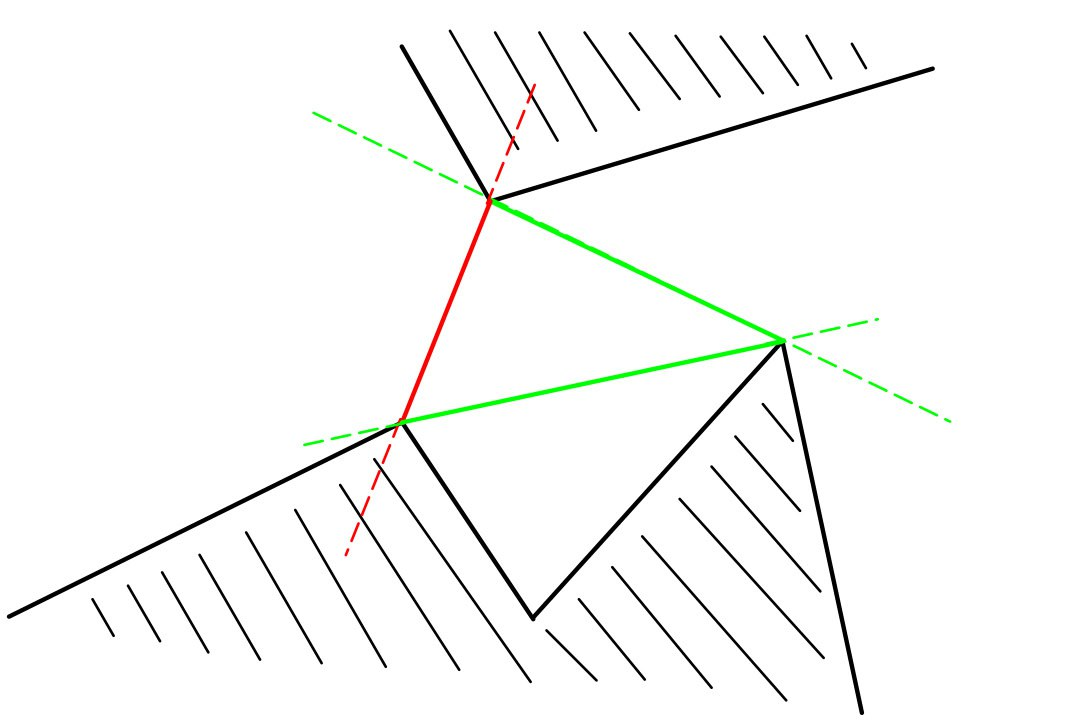
\includegraphics[width=0.6\linewidth]{images/5.png}
    \caption{Незначащее ребро}
    \label{fig:minor_edge}
\end{figure}


\end{theorem}

Дополнительные оптимизации, следующие из геометрических соображений:

\begin{enumerate}
    \item Можно заметить следующее: если имеются две вершины $u$ и $v$ такие, что первая из них расположена ниже второй
        (то есть ее $y$-координата меньше), тогда при обработке вершины $v$ в качестве источника ребро $(u,v)$
        уже было бы добавлено (если оно допустимо) на шаге обработки вершины $u$. Следовательно, можно исключить 
        из рассмотрения все вершины $u$, $y$-координата меньше $y$-координаты текущей вершины-источника $v$.
    
    \item Рассмотрим три последовательные вершины $\operatorname{prev}(\mathit{cur})$, $\mathit{cur}$ и $\operatorname{next}(\mathit{cur})$. 
    Если эти вершины образуют поворот по часовой стрелке, то вершина $\mathit{cur}$ является вогнутой, 
    и все инцидентные ей ребра в графе видимости являются незначащими согласно теореме~\ref{thm:minor_edge} (рис. \ref{fig:concave}). 
    Следовательно, такая вершина $\mathit{cur}$ может быть полностью исключена из рассмотрения в качестве кандидата на проведение ребер.
    \begin{figure}[H]
        \centering
        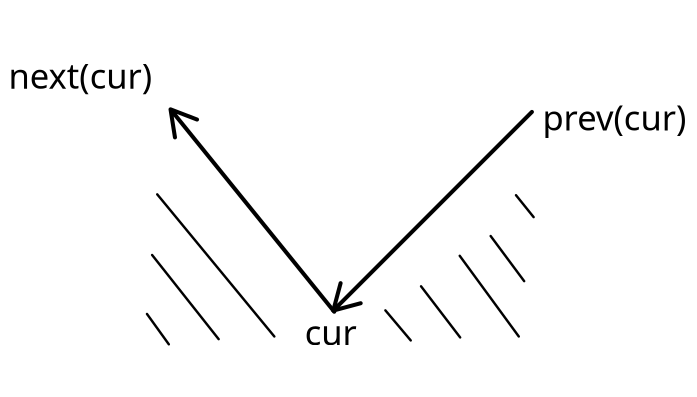
\includegraphics[width=0.6\linewidth]{images/2.png}
        \caption{Вогнутая часть препятствия}
        \label{fig:concave}
    \end{figure}
    
    \item Если же указанные вершины образуют поворот против часовой стрелки, то вершина $\mathit{cur}$ является выпуклой. 
    В этом случае при обработке вершины $\mathit{cur}$ все ребра, построенные в вершины, лежащие внутри сектора, 
    образованного лучом из $\operatorname{prev}(\mathit{cur})$ через $\mathit{cur}$ и лучом из $\operatorname{next}(\mathit{cur})$ через $\mathit{cur}$, 
    будут незначащими (рис. \ref{fig:convex}). Данное множество вершин может быть исключено из проверки видимости.

    \begin{figure}[H]
        \centering
        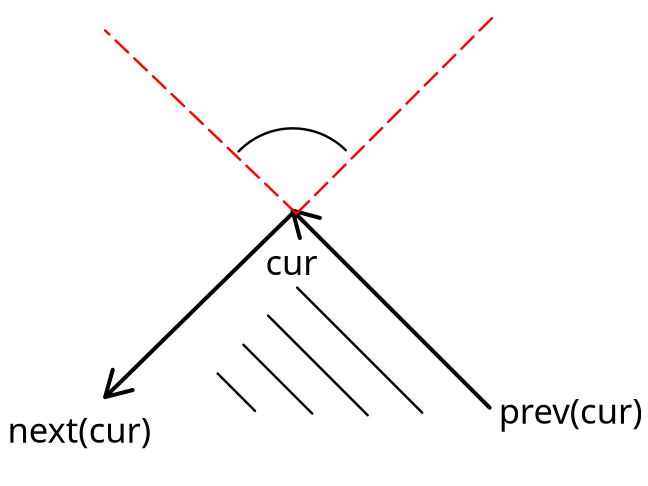
\includegraphics[width=0.6\linewidth]{images/1.png}
        \caption{Выпуклая вершина $\mathit{cur}$. Рёбра, проведённые из неё в вершины, лежащие внутри красного сектора, являются незначащими.}
        \label{fig:convex}
    \end{figure}
    
\end{enumerate}

В реализации последняя оптимизация может оказаться сложнее остальных.
Например, можно действовать следующим образом:
\begin{enumerate}
   \item Применять стандартный алгоритм Ли для источника, но лишь до тех пор, пока заметающий луч не доходит до границы сектора,
       образованного лучами $[\operatorname{prev}(\mathit{cur}), \mathit{cur})$ и $[\mathit{cur}, \operatorname{next}(\mathit{cur}))$, 
       как показано на рис.~\ref{fig:convex} красным цветом (т.~е. не совершает полный оборот).
    \item Применять следующую модификацию алгоритма Ли:
        \begin{itemize}
            \item Луч $L$ устанавливается в направлении горизонтально влево (при условии, что применен п. 1).
            \item В статус аналогично вносятся все ребра препятствий, которые пересекает луч в этом начальном положении,
                  упорядоченные по расстоянию от источника.
            \item События обрабатываются в порядке убывания полярного угла.
        \end{itemize}
    \item Обработка продолжается до достижения другой границы сектора.
\end{enumerate}
В результате вершины, находящиеся внутри этого сектора, не обрабатываются, что позволяет существенно
сократить время работы алгоритма.

Можно заметить, что обработка различных вершин в качестве источников происходит независимо, 
поскольку для каждого источника рассматриваются вершины только с большей координатой $y$ (согласно п. 1). 

Это свойство позволяет эффективно распараллелить вычисления. Список отсортированных вершин можно обрабатывать параллельно. 

Для параллельной обработки множество вершин-источников разбивается на непересекающиеся подмножества (пакеты),
которые распределяются между потоками. Такая пакетная обработка (chunking) минимизирует накладные расходы на
синхронизацию и балансирует нагрузку, обеспечивая масштабирование производительности пропорционально числу доступных ядер процессора.

\section{ХРАНЕНИЕ ГРАФА}

В вычислительных задачах, связанных с графами, важную роль играет выбор способа их хранения.
В то время как с теоретической точки зрения очевидным выбором является
хранение списков смежности при каждой вершине графа, реализация
схемы представления этих списков смежности в оперативной памяти
является важной деталью реализации.

\subsection{Наивная схема хранения}
Наиболее простым подходом 
является хранение для каждой вершины контейнера с инцидентными ей рёбрами или соседними вершинами. 
Наивная реализация такого подхода может выглядеть следующим образом:

\begin{lstlisting}[language=C++]
struct Vertex 
{
    std::forward_list<edge_id> edges;
};

struct Edge 
{
    vertex_id a;
    vertex_id b;
};
\end{lstlisting}

\subsection{Реализация в Boost Graph Library (BGL)}

Общедоступная библиотека BGL имеет шаблонизированный класс \texttt{adjacen\-cy\_list}~\cite{BGLadj}, предоставляющий разные варианты хранения списка вершин и списков рёбер:
\texttt{vector}, \texttt{list}, \texttt{slist} (односвязный список), \texttt{set}, \texttt{multiset}, \texttt{unordered\_set}. Быстродействие
различных операций с графом зависит от того, какие контейнеры используются. Также существует гибкая схема (т.~н. «custom storage»), в рамках
которой программист может определить свои контейтеры для представления списков смежности.

При большом количестве вершин возникает проблема фрагментации памяти
из-за обилия небольших фрагментов памяти, выделенных в
куче. Фрагментация памяти приводит к возросшему количеству «промахов»
кеша процессора и к общему снижению производительности
программы. Для борьбы с фрагментацией теоретически можно использовать
вышеупомянутую возможность создания специальных контейнеров, однако
публично доступные примеры таких контейнеров неизвестны. Альтернативой
в BGL является «компрессированная» форма представления графа в памяти
— Compressed Sparse Row, CSR~\cite{BGLCSR}, ограничением которой является
невозможность модификации графа.

\subsection{LogGraph}

Ещё одной «компрессированной» формой представления графа в памяти
является LogGraph~\cite{LogGraph} — достаточно сложная схема,
близкая к оптимальной по степени компрессии и имеющая сравнительно
невысокие накладные расходы на декомпрессию. Как и CSR, LogGraph
предназначена для хранения в оперативной памяти статичных, не
модифицируемых графов.

\subsection{Реализации в LEMON и Indigo}

LEMON (Library for Efficient Modeling and Optimization in Networks)~\cite{LEMON}
--- библиотека для работы с графами, в настоящее время не развиваемая
(разработка происходила в 2004--2014 гг.). Это наиболее ранняя
найденная авторами (и одна из немногих) реализация хранения списков
смежности всех вершин в едином контейнере, что позволяет избежать
фрагментации памяти (при этом, в отличие от вышеупомянутой схемы CSR,
возможна модификация графа).
Данная реализация доступна в виде исходного кода и не документирована.

Аналогичное решение применено в Indigo — библиотеке для работы с
молекулярными структурами~\cite{Indigo,IndigoGithub}. Односвязные списки смежности всех вершин
графа хранятся в едином контейнере под названием «пул» (pool), который
в свою очередь реализован на массиве. Данная реализация также доступна в
виде исходного кода и не документирована.

В настоящей работе наряду с «наивной» схемой хранения список смежности
реализована схема хранения, аналогичная реализациям в LEMON и Indigo.
Эта схема не претендует, подобно CSR и LogGraph, на оптимальность
по объёму памяти, но тем не менее устраняет проблему фрагментации,
при этом позволяя добавление и удаление вершин и рёбер.

\section{РЕЗУЛЬТАТЫ ТЕСТИРОВАНИЯ ПРОИЗВОДИТЕЛЬНОСТИ}

В качестве результатов сравним время работы наивного алгоритма и оптимизированного алгоритма Ли.

\subsection{Тестовые данные}

Тестирование проводилось на наборе полигональных препятствий, построенных на основе данных 
электронной навигационной карты из открытого источника NOAA~\cite{NOAA}. Карта представляет собой береговую
линию (изобата нулевой глубины). Внешняя граница области также включена в состав препятствий, 
что делает сцену ограниченной. Результирующая сцена изображена на рис.~\ref{fig:test_graph}.
Характеристики сцены: общее количество вершин препятствий $n = 6578$. Изолированные вершины отсутствуют, поэтому количество рёбер 
препятствий также равно 6578.

\begin{figure}[H]
    \centering
    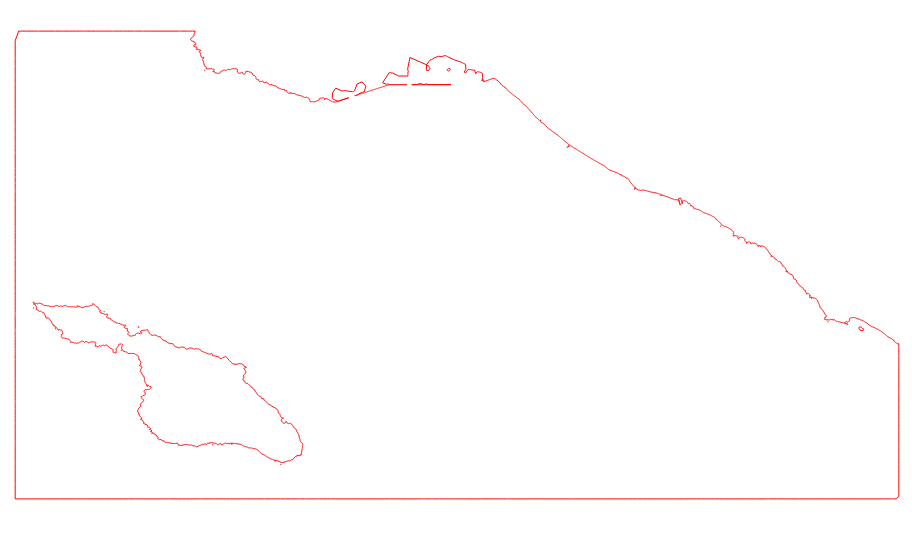
\includegraphics[width=0.6\linewidth]{images/3.png}
    \caption{Исходный планарный граф}
    \label{fig:test_graph}
\end{figure}

Количеств рёбер в построенном графе видимости равно 12668. Граф видимости
изображён на рис.~\ref{fig:visibility_graph}.

\begin{figure}[H]
    \centering
    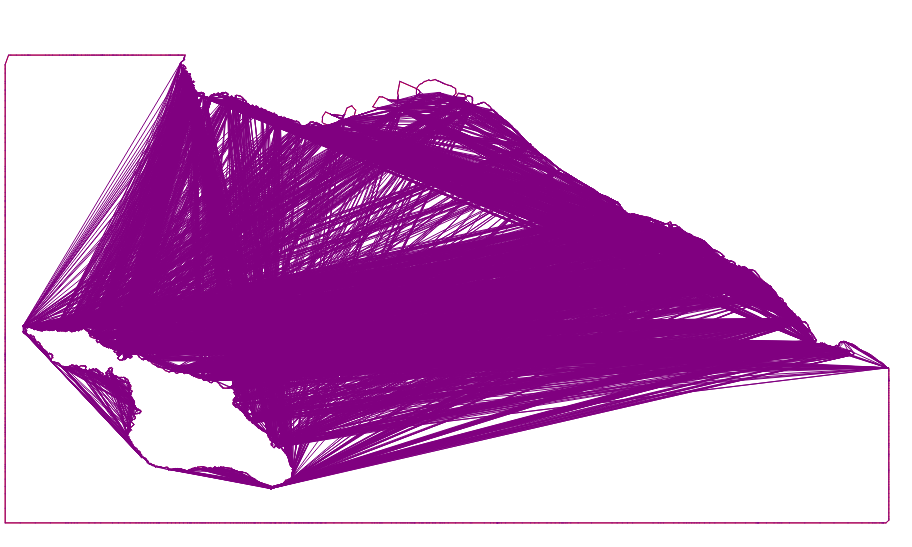
\includegraphics[width=0.6\linewidth]{images/4.png}
    \caption{Построенный граф видимости}
    \label{fig:visibility_graph}
\end{figure}

\subsection{Характеристики тестового оборудования}

Тестирование проводилось на машине со следующими характеристиками:
\begin{itemize}
    \item процессор: AMD Ryzen 5 5600X 6-Core Processor;
    \item тактовая частота: базовая 2.2 ГГц, максимальная 4.65 ГГц;
    \item оперативная память: 32 ГБ;
    \item операционная система: Ubuntu 24.04.4 LTS.
\end{itemize}

\subsection{Результаты замеров времени}

В Табл.~\ref{tab:results} представлены результаты замеров времени работы различных реализаций алгоритмов.

\begin{table}[H]
    \centering
    \caption{Сравнение времени работы алгоритмов}
    \label{tab:results}
    \small
    \begin{tabular}{|p{9cm}|c|}
        \hline
        \textbf{Алгоритм} & \textbf{Время выполнения, с} \\
        \hline
        Наивный алгоритм (O(n²·m)) с фрагментированным представлением графа & 28.401 \\
        \hline
        Наивный алгоритм (O(n²·m)) с дефрагментированным представлением графа  & 26.074 \\
        \hline
        Алгоритм Ли без оптимизаций & 4.786 \\
        \hline
        Алгоритм Ли с оптимизациями и фрагментированным представлением графа & 1.003 \\
        \hline
        Алгоритм Ли с оптимизациями и дефрагментированным представлением графа & 0.963 \\
        \hline
        Алгоритм Ли с оптимизациями, дефрагментированным представлением графа и распараллеливанием & 0.340 \\
        \hline
    \end{tabular}
\end{table}

Отметим, что дефрагментированное представление графа ускоряет работу наивного алгоритма на 9\%,
а работу оптимизированного алгоритма Ли на 4\%.

\section*{ЗАКЛЮЧЕНИЕ}

В результате проделанной работы удалось значительно ускорить алгоритм Ли для построения графа видимости.
Были реализованы и протестированы наивный алгоритм, алгоритм Ли, оптимизированная версия алгоритма Ли, а также его параллельная модификация.
Эксперименты на сцене с 6578 вершинами показали, что оптимизированный алгоритм работает более чем в 25 раз быстрее наивного,
а распараллеливание на 12 потоков даёт дополнительное ускорение в 2.5 раза.

Дефрагментация представления графа в оперативной памяти даёт дополнительный прирост производительности 
за счет меньших накладных расходов при доступе к данным.

Полученные результаты могут быть использованы в системах планирования пути, работающих в реальном времени,
и в других прикладных задачах, связанных с вычислительной геометрией.

\additionalinfo{Поступила в редакцию \today, окончательный вариант \today}

\printauthorsinfo

\bibliographystyle{ugost2008}
\bibliography{references-clones}

\begin{translatedpart}
    \englishversion
    
    \maketranslatedtitle

    \begin{abstract}
        \insertabstract
        \insertkeywords
        \autocitationexample
    \end{abstract}
    
    \begin{otherlanguage*}{english}
            \bibliographystyleeng{IEEE} 
            \bibliographyeng{references-en,references-clones}

    \end{otherlanguage*}
    \additionalinfo{\selectlanguage{english}Received \today, final version \today}
    
\end{translatedpart}   

\end{document}
